\chapter{Desarrollo de la solución}
A la hora de empezar con la implementación de la solución, debemos comenzar teniendo en cuenta la arquitectura software que satisface requisitos del sistema de acuerdo con los usuarios. Es decir, con las historias de usuario que han expresado.

\section{Arquitectura software de la solución}
Para el diseño del software se ha utilizado el diseño dirigido por el dominio, DDD \textit{Domain Driven Design}. Este tipo de arquitectura introducida por Eric Evans \cite{ddd_book} "Domain-Driven-Design - Tackling Complexity in the Hearth of Software, 2004" nos permite organizar el código de forma separada y organizada lo que nos permite poder realizar TDD correctamente ya que por tener las distintas capas separadas y débilmente acopladas unas de las otras. Gracias a este bien diseño es muy fácil hacer uso de la inversión de dependencias \footnote{https://jj.github.io/curso-tdd/temas/inversi\%C3\%B3n.html} para inyectar en los tests las clases \textit{mockeadas} \footnote{El término mockear en desarrollo de software se refiere a reemplazar o imitar a un objeto real. El propósito es que al probar el programa o hacer testing, podamos utilizar este mock para conocer su estado.} que necesitemos. 

La arquitectura dirigida por el dominio nos permite fácilmente aislar la lógica de negocio en un único sitio y siempre lo más cerca del dominio posible lo que nos permite cumplir los principios SOLID fácilmente y conseguir un código abierto a su extensión pero cerrado a su modificación.  

Un requisito fundamental expresado por los usuarios diana a utilizar este proyecto es poder desplegar fácilmente este proyecto en la nube, gracias a que se ha desarrollado utilizando capas desacopladas entre si, podemos distribuir en distintos clústeres \footnote{Nos referimos a la técnica por la cual podemos combinar un sistema para que trabaje paralelamente en un entorno cloud. Lo que conseguimos con esta operación es una mayor disponibilidad, más velocidad de despacho y escalabilidad del sistema. Como todo, a cambio tendremos un sistema más costoso de mantener económicamente y un mayor tiempo de implementación. } la implementación sin realizar prácticamente cambios en la implementación.  Es fundamental desacoplar al máximo todos los componentes y que cada uno tengo una única responsabilidad cuando se realiza un proyecto en la nube. La principal desventaja que podemos encontrar en este tipo de arquitecturas es la comunicación entre los distintos componentes.  Una solución a este problema podría ser la comunicación por eventos, potente pero compleja a nivel técnico y costosa económicamente. Otra solución es mediante inyección de dependencias, que es la que he empleado en este proyecto, podemos decir que la debilidad de esta solución reside en que una de las capas puede crecer en sobremedida y convertirse en un cuello de botella.



\subsection{DDD}
En este tipo de arquitectura donde diseñamos guiándonos por el dominio, podemos diferenciar tres elementos importantes.

\subsubsection{Entidad}
Las entidades son aquellas clases que representan una entidad del dominio. Estas clases deben tener una estructura de datos que represente la información de la entidad y unas responsabilidades concretas. Se caracterizan porque tienen que ser consideradas iguales a otros objetos aún cuando cuando sus atributos difieren. En las entidades se encuentran las restricciones del dominio, en ellas se realizan las validaciones de valor e integridad. Cualquier error o situación inválida hay que notificársela al sistema mediante una excepción. 

Definir y diseñar los estados inválidos de las entidades y de la aplicación en general es un apartado fundamental que debemos de realizar con el mismo cuidado que con el que diseñamos las entidades.

Este proyecto consta de dos entidades: \codeword{Disease} que representa a una enfermedad y \codeword{Raziel} que es sin lugar a duda el modelo más rico en información. Estas entidades poseen las restricciones de valor como puede ser el tipado de sus atributos o la satisfacibilidad solo de los valores que tienen sentido semántico. También restricciones de integridad como por ejemplo, que un objeto de tipo \codeword{Disease} puede tener el campo \codeword{cie}, nulo.

\subsubsection{Value objects}
Representan los conceptos que no tienen una entidad. Describen características por lo que solo nos interesan sus atributos.
Los value object representan elementos del modelo que se describen por el \textbf{qué} son, y no por \textbf{quién} o \textbf{cuál} son. Estos elementos completan y/o forman parte de las entidades del sistema.

En este proyecto la representación en código de las comunidades autónomas corresponde con un tipo de value object utilizado por la entidad \codeword{Raziel}

\subsubsection{Servicios}
No tienen significado propio suponen la capa que representa las operaciones que no pertenecen conceptualmente a ningún objeto del dominio concreto. 

En este proyecto, los servicios son el punto de entrada de las peticiones que le hace el usuario al sistema. Son también los encargados de arrancar todo el proceso de obtención de los datos.

\subsubsection{Repositorios}
Representan al conjunto de modelos y entidades. Se utilizan para almacenar u ofrecer los conjuntos de objetos. Suelen suponer una capa de abstracción sobre el sistema de almacenaje, ya sea una base de datos, unos ficheros en disco o incluso la invocación de otros servicios externos como puede ser un API. Esta parte es fundamental para poder modular y preparar las aplicaciones para cambiar de infraestructura sin tener que modificar el código de programación.

En este proyecto hemos implementado este concepto haciendo uso de un \codeword{AbstractRepository} representado por una clase abstracta. Debido a que, semánticamente no tiene sentido poder utilizar este tipo de repositorio en sí mismo. Sin embargo, es usado de clase padre para el resto de repositorios porque impone a las clases que lo heredan una interfaz uniforme de métodos y abstrae lógicas comunes a este tipo de concepto.

El proyecto está compuesto por cinco repositorios que obtiene en forma sus modelos correspondientes. Al existir este tipo de jerarquía y compartir todos estos el mismo tipo de operación, resulta idónea la aplicación del patrón de diseño de creación \textit{Factory Method}. Si bien es cierto, que es en lenguajes tipados donde este tipo de soluciones suponen un cambio radical en cuanto a la comodidad y encaje en la creación de instancias a lo largo del programa. A nosotros también nos mejora la calidad del código, pudiendo hacer uso de cualquier repositorio con una sola importación, ya que en otro caso habría que construir el repositorio \textit{in situ} e inyectarle todas las dependencias que necesitara.


\subsection{Diagrama arquitectónico de la solución}
A continuación se puede ver un somero diagrama donde podemos observar la conexión entre los distintos componentes del sistema y la conexión con librerías y frameworks externos. 

\begin{figure}[]
	\centering	
	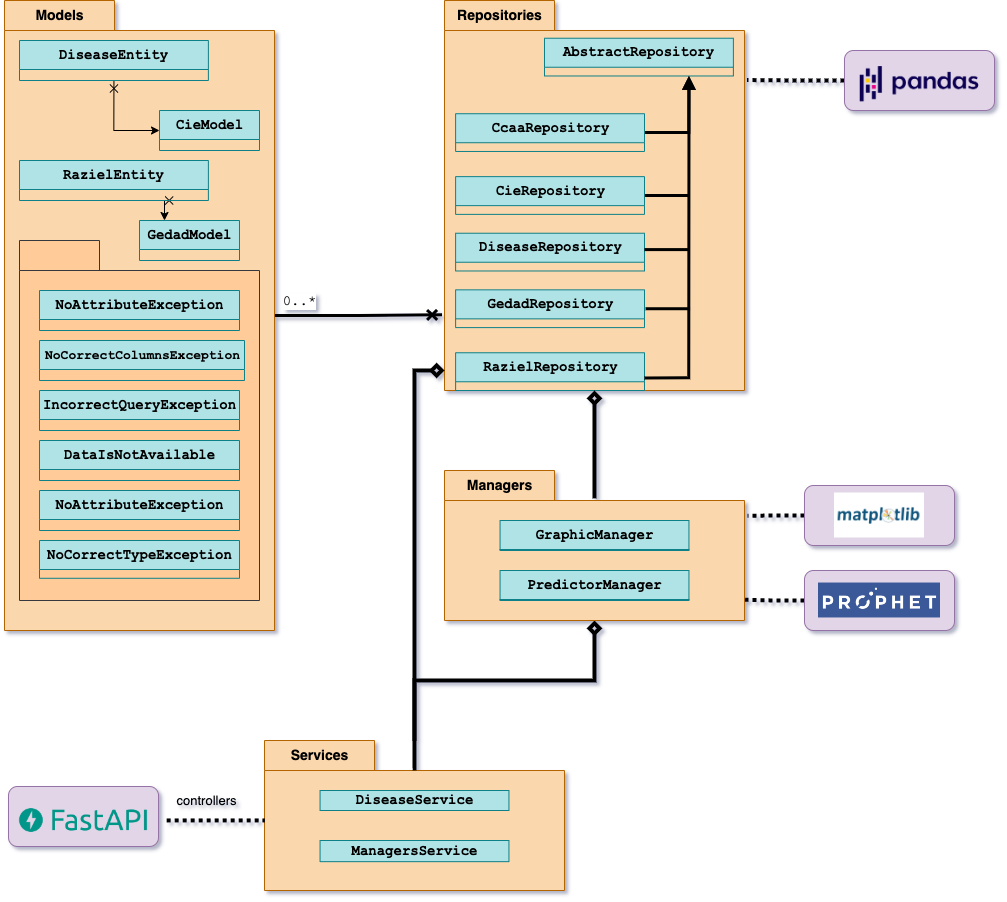
\includegraphics[scale=0.5]{doc/logos/imgs/arquitectonico.png}
	\caption{ \cite{rtve-cis} Modelo organizativo del código con sus dependencias externas. }
    \label{fig:worst_f_value}
\end{figure}



\section{Implementación}
\subsection{Lenguaje de programación}
El lenguaje elegido ha sido \textbf{Python} los motivos de esta decisión son variados, por los que procedo a enumerarlos:
\begin{itemize}
    \item Es un lenguaje que se encuentra en las \cite{tiobe} primeras posiciones como lenguaje más utilizado a día de hoy. Además me encuentro muy cómodo programando en él.
    \item Es un lenguaje que cuenta con muchísimas bibliotecas, muchas de estas especiales para trabajar con datos y ficheros (como \textbf{Pandas}). Abundan también los \textit{frameworks} que nos ayudan a construir APIs con él y la mayoría de PaaS \footnote{Platform as a Service} soportan este lenguaje.
    \item Es un lenguaje interpretado, débilmente tipado y con una capacidad introspectiva muy alta que nos permite metaprogramar.
\end{itemize}

A la hora de realizar un proyecto software siempre es necesario utilizar bibliotecas y código implementado por otras personas para poder llegar más lejos. Todo esto es lo que llamamos dependencias. Muchos entornos de programación tienen gestores de dependencias que nos permiten instalar y gestionar estas dependencias cómodamente. En el entorno JavaScript tenemos \textit{npm} o \textit{yarn} que nos permite instalar dependencias de forma sencilla. Para la JVM el tradicional \textit{maven} es una buena opción o la mas moderna y potente \textit{Gradle}.

En Python se ha extendido el uso de \textbf{Poetry} que de forma muy parecida a \textit{npm} genera un fichero de configuración \textit{pyproject.toml} donde definimos las dependencias, las versiones y los paquetes de nuestro proyecto así como algunas tareas específicas para correr los tests o el lint fácilmente. Esto facilita enormemente la creación de entornos virtuales de prueba y de desarrollo tanto el local como por el CI.

\subsection{Bibliotecas utilizadas}

\section{Para Continuos Integration}
Desde el inicio del trabajo se ha estado trabajando con un sistema férreo de CI de forma que no se ha mezclado nunca nada que no haya superado los requisitos de diseño especificados. En el entorno de desarrollo se ha utilizado \textit{Github Actions} que es una herramienta de CI que nos permite realizar una integración continua de la misma forma que \textit{Travis CI} la elección de Github sobre Travis es por la rapidez del elegido e integración con la forja utilizada que como se ha especificado anteriormente es Github.

Para garantizar la \textbf{calidad de la memoria} se han implementado dos tipos de CI\footnote{Continuos Integration}: un revisor ortográfico y un revisor de estructura que compila el documento automáticamente y pública el PDF generado en las \href{https://github.com/pablojjimenez/TFG/releases}{\textit{releases} del repositorio.}

Del mismo modo, para el \textbf{código} se han implementado otras dos CI que garantizan que cuando se introduce en la rama principal del repositorio código nuevo, éste garantiza unos estándares de calidad y que efectivamente el código es funcional por todas las versiones especificadas de Python. Por un lado, verificar el código fuente contra errores de programación (como "library imported but unused" y "Undefined name") y para verificar la complejidad ciclomática. Se ha utilizado la tecnología \cite{flake}\textbf{Flake8} por ser las más utilizada en el ecosistema.
Por otro lado, se corre la \textit{suit} de tests de forma que se garantice que al añadir uno código no se rompe el existente. Se ha utilizado la librería \textit{Unittest} que se encuentra incluida en la biblioteca estándar de Python permite realizar aserciones, provee de muchas aserciones y permite organizar los tests de forma parecida a como lo hace jUnit en clases que llamamos \textit{suits} de tests.

Todas estas comprobaciones se realizan para todas las versiones de Python en las que garantizamos que el software funciona.

\subsubsection{Pandas}
Como se ha descrito en anteriores capítulos de la memoria, los datos que manejamos están en ficheros CSV. Para poder trabajar con ellos es necesario utilizar una biblioteca que nos permite trabajar con estos ficheros. Es necesario poder manejar los datos de estos ficheros con cierta agilidad. El mayor fichero tiene 967360 líneas y ocupa unos 55 MB aunque no son cifras cercanas a lo que se considera \textit{big data} necesitamos de una herramienta que nos permita filtrar, ordenar y hacer cálculos eficientemente sobre estos conjuntos de datos. La elección de \textbf{Pandas} como biblioteca para trabajar con estos datos es debido a que es ampliamente utilizada en el mundo Python y encaja en los datos que tenemos.

\subsubsection{Matplotlib}
Es una biblioteca para crear todo tipo de gráficos, es muy utilizada en el ecosistema Python y además ha sido elegida por su compatibilidad con \textit{Pandas} que permite realizar gráficas a partir de objetos Dataframe propios de la biblioteca \textit{Pandas}

\subsubsection{Prophet}
Es necesario poder obtener predicciones basadas en series temporales. Busco que la predicción sea rápida. Sea automática de forma que no haya que configurar muchos parámetros y que el pronóstico que ofrece sea ajustable; esto es, que permita modificar y ajustar los pronósticos agregando conocimiento del dominio.

La primera opción y más famosa en el lenguaje Python es scikit-learn, una biblioteca open source de machine learning que ofrece infinidad de algoritmos: de clasificación, regresión, clustering, selección de modelos, preprocesado...

Por otro lado, tenemos Prophet una biblioteca open source para Python y R desarrollada por Meta. Sus posibilidades son mas limitadas que las que nos ofrece scikit-learn pero por el contrario es muy básica y sencilla tanto de instalar como de usar. Además, su funcionalidad es justo la que buscamos, poder realizar predicciones sobre series temporales.

En Prophet, los modelos se ajustan usando Stan, otra biblioteca de inferencia estadística bayesiana con estimación de verosimilitud penalizada.

\subsubsection{FastAPI}
En aras de que el usuario pueda utilizar estos servicios de forma agnóstica sin tener que descargarse el código fuente e incluirlo en su proyecto a modo de biblioteca. Algo que por otra parte, supondría una gran restricción ya que el lenguaje de programación tendría que ser Python.

Para ello, se ha implementado una interfaz de comunicación REST. Como bien es sabido, los servicios restful se apoyan del estándar HTTP y por tanto, hereda sus conocidas características. REST es \textit{stateless} cada vez que utilizamos un recurso necesitamos ofrecerle toda la información identificativa pues carece de memoria, utiliza el formato JSON para el intercambio de datos y expone una serie de recursos o \textit{endpoints} que son las operaciones disponibles a realizar.

En el universo Python existen dos grandes frameworks para construir servicios restful: Flask y FastAPI.
Flask es un microframework, que dispone de multitud de complementos lo que te permite construir cualquier servicio configurando correctamente todos estos complementos. 

FastAPI es un proyecto de código libre mas moderno, de alto rendimiento, según la documentación \footnote{https://fastapi.tiangolo.com} oficial se podría igual al rendimiento que ofrece NodeJS o Go. Además, nos permite por defecto programar de forma asíncrona (muy interesante cuando hay acceso a bases de datos) y nos proporciona de forma automática una documentación OpenAPI.

La API de este software expone dos blueprints \footnote{Llamamos blueprint al conjunto de recursos que comparte el mismo prefijo de URI (Identificador de recursos uniforme)}

\begin{itemize}
    \item \textit{/data} Definido por el conjunto de recursos disponibles. Todos ellos aceptan los siguientes parámetros en la cabecera de las peticiones \codeword{sort} para ordenar los datos en base a algún campo, \codeword{limit} para limitar la cantidad de datos (por defecto se entregan limitados a 100 elementos), \codeword{page} para especificar la página.
    Y la siguiente estructura JSON como cuerpo de la petición:
    \begin{verbatim}
        {
            "ID": {
                ">": 1,
                "<": 3
            },
            "CIE": {
                "==": ""
            }
        }
    \end{verbatim}
    En este caso estaríamos indicando que queremos los elementos cuyos IDs se encuentran en el rango ]1, 3[ y cuyo campo CIE es vacío. Los operadores válido son: \codeword{==}, \codeword{<}, \codeword{>}

    \item \textit{/managers} Dispone de tres recursos. Uno para generar gráficos lineales (ver figura): requiere dos variables como parámetros en la cabecera, una para indicar la agrupación y otra para la suma, como cuerpo de la llamada podemos pasar una query con la estructura especificada anteriormente. Por último, tenemos dos recursos para obtener la predicción y la gráfica ajustada en el tiempo que indiquemos.
\end{itemize}

\subsubsection{Documentación de la API}
Con la ayuda de los recursos que pone a nuestra disposición FastAPI, se ha implementado una especificación OpenAPI. Esta especificación define una serie de propiedades en un formato legible por una máquina (suele usarse el formato JSON o YAML).

Gracias a eso podemos generar una documentación basada en HTML que nos permite conocer los recursos expuestos de la API, los argumentos y las estructuras de las respuestas esperadas. Los modelos están documentados en el código para los usuarios que decidan utilizar el software como biblioteca puedan ver dicha documentación en el IDE que utilicen. Para aquellos que utilicen la API, se ha añadido a la especificación OpenAPI

\begin{figure}[]
	\centering	
	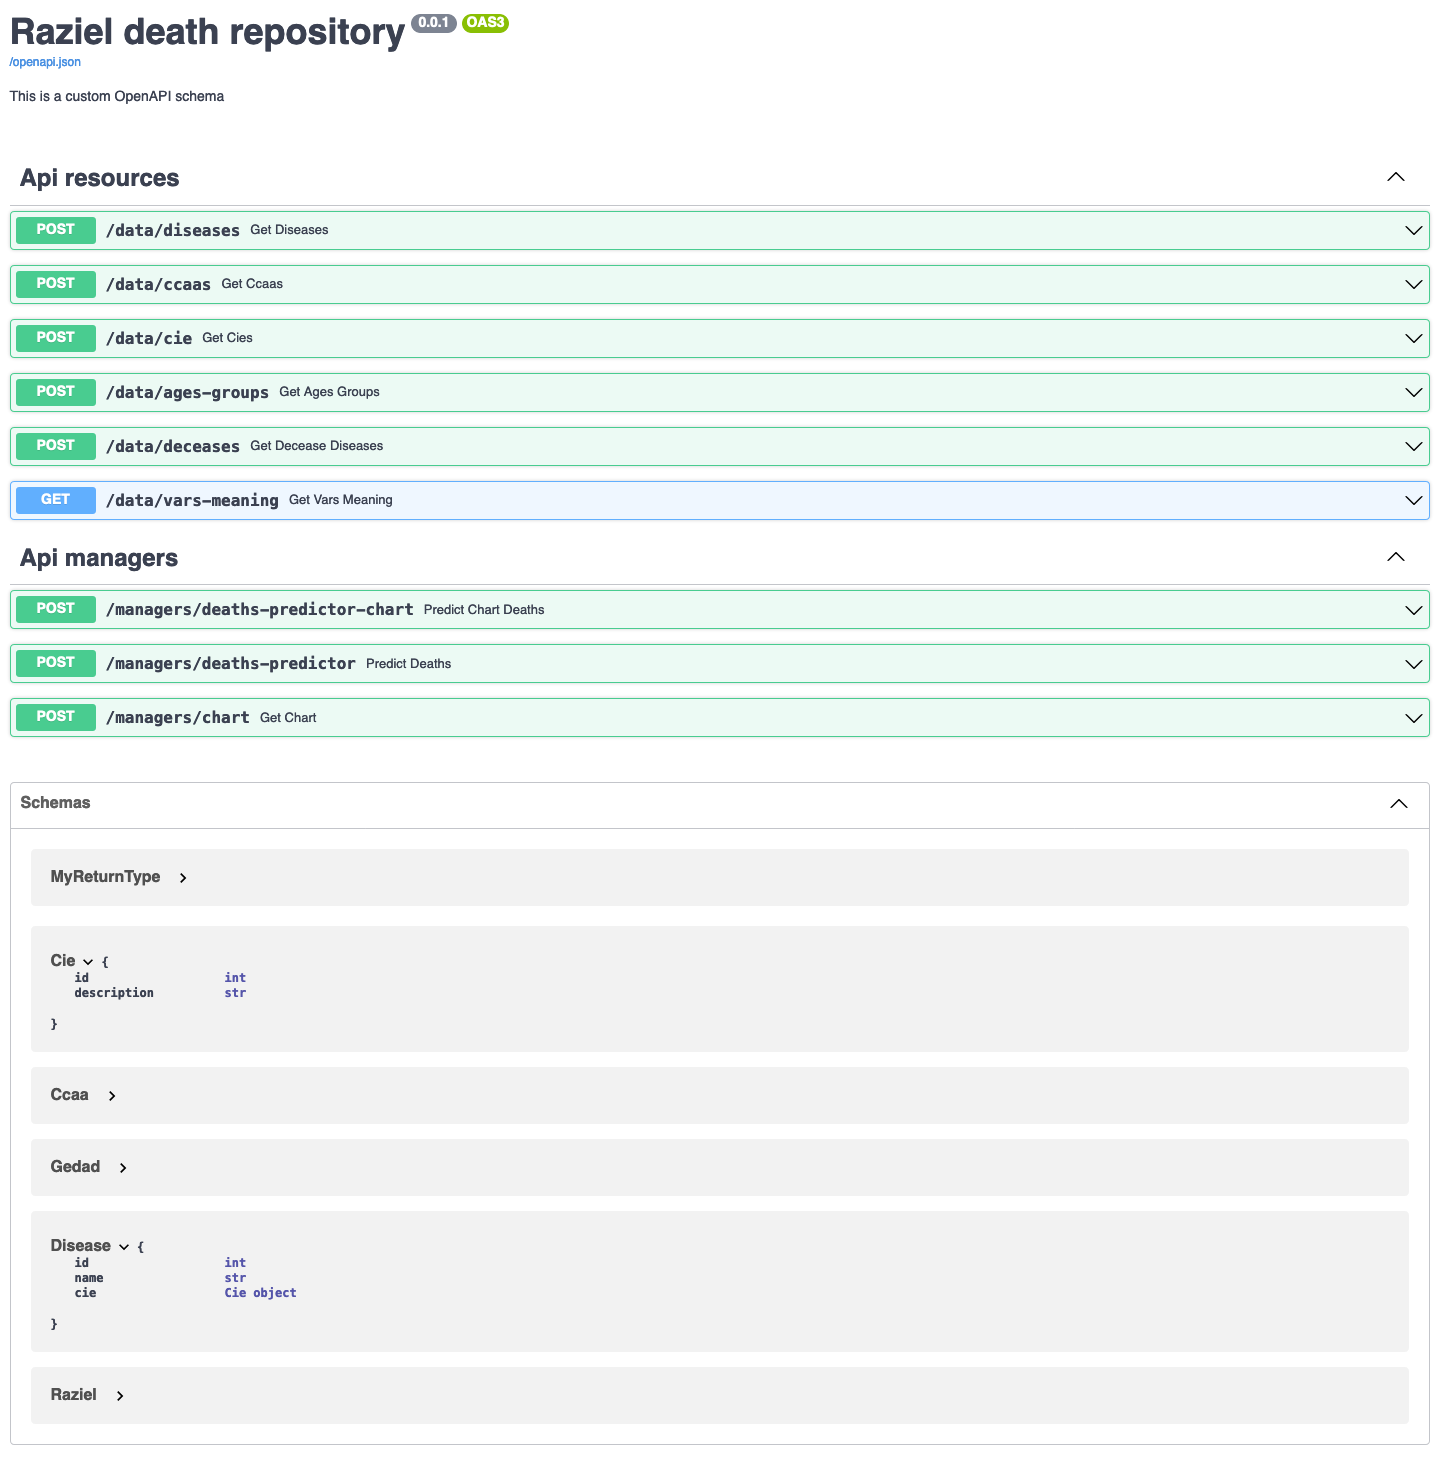
\includegraphics[scale=0.5]{doc/logos/imgs/openapi.png}
	\caption{ \cite{rtve-cis} Documentación OpenAPI de la API. }
    \label{fig:worst_f_value}
\end{figure}